\documentclass[Master,ngerman,UKenglish]{scrbook}
%------------------------------------------------------------------------------
% This file contains a skeleton thesis for
% a Physics or Astronomy Institute in the University of Bonn

% Specify the thesis type as an option: PhD, Master, Diplom, Bachelor
% Specify the thesis stage as an option: Draft (default), Submit, Final, PILibrary

% Specify the language(s) in the class and then use babel.
% If you need more than one language, give the default language last,
% e.g. ngerman,UKenglish for a thesis in British (UK) English where you want
% to be able to set the language to German for some part of it.

%------------------------------------------------------------------------------
% Pass TeX Live version to the package
% Use command pdflatex --version to find out which version you are running
% Add option backref=false when your thesis is ready to turn off back-referencing
% in your bibliography
\usepackage[texlive=2014,astrobib]{ubonn-thesis}
% Adjustments to standard biblatex style
\usepackage{ubonn-biblatex}

% Glossary package
% \usepackage[acronym,toc,nosuper]{glossaries}
% TikZ packages and libraries
% \usepackage{tikz}
% \usepackage{tikz-3dplot}
% \usepackage{pgfplots}
% \usetikzlibrary{positioning,shapes,arrows}
% \usetikzlibrary{decorations.pathmorphing}
% \usetikzlibrary{decorations.markings}
\usepackage{thesis_defs}

%------------------------------------------------------------------------------
% Instead of colouring  links, cites, table of contents etc.
% put them in a coloured box for the screen version.
% This is probably a good idea when you print your thesis.
% \hypersetup{colorlinks=false,
%   linkbordercolor=blue,citebordercolor=magenta,urlbordercolor=darkgreen
% }

%------------------------------------------------------------------------------
% When writing your thesis it is often helpful to have the date and
% time in the output file. Comment this out for the final version.
\ifoot[\today{} \thistime]{\today{} \thistime}

% In order to check if your labels are referenced try the refcheck package
% \usepackage{refcheck}

%------------------------------------------------------------------------------
% biblatex is included by ubonn-thesis. Look there for the settings used.
% See the options for settings that can be changed easily.
% For further changes copy the \RequirePackage[...]{biblatex} here
% and include ubonn-thesis with the option biblatex=false.

% Specify the bibliography files here and not at the end!
% Use standard_refs-bibtex if you use bibtex or bibtex8
% and standard_refs-biber  if you use biber
\addbibresource{thesis_refs.bib}
\addbibresource{../refs/standard_refs-biber.bib}

% You can include the following lines if you want to shorten your
% bibliography by not including url fields
% \AtEveryBibitem{\clearfield{url}}
% \AtEveryCitekey{\clearfield{url}}

%------------------------------------------------------------------------------
% The following definitions are used to produce the title pages
% needed at various stages
\newcommand{\thesistitle}{Title of the Thesis}
\newcommand*{\thesisauthor}{Author's name}
\newcommand*{\thesistown}{Place of birth}
\renewcommand*{\InstituteName}{\AIFA}
\renewcommand*{\inInstitute}{\inAIFA}
\renewcommand*{\InstituteAddress}{\PIaddress}
% Adjust \thesisreferee...text depending on male/female referee
\newcommand*{\thesisrefereeonetext}{1.\ Gutachter}
\newcommand*{\thesisrefereeone}{Prof.\ Dr.\ John Smith}
\newcommand*{\thesisrefereetwotext}{2.\ Gutachterin}
\newcommand*{\thesisrefereetwo}{Prof.\ Dr.\ Anne Jones}
% Date when thesis was submitted (Master/Diplom)
% Year or Month, Year when thesis was submitted (PhD)
\newcommand*{\thesissubmit}{XX.YY.2016}
% \newcommand*{\thesissubmit}{Month 2016}
% Date of thesis examination (PhD)
\newcommand*{\thesispromotion}{XX.YY.2016}
% Month and year of the final printed version of the thesis
\newcommand*{\thesismonth}{MMM}
\newcommand*{\thesisyear}{2016}
\newcommand*{\thesisnumber}{BONN-IR-2016-XXX}

%------------------------------------------------------------------------------
% The abstract is only needed for the printed version and should be in
% English regardless of the language of the thesis
\newcommand{\thesisabstract}{%
  \begin{otherlanguage}{UKenglish}
    This is your thesis abstract. It may be in a language that is
    different from the rest of your thesis.
  \end{otherlanguage}
}

%------------------------------------------------------------------------------
% \includeonly can be used to select which chapters you want to process
% A simple \include command just inserts a \clearpage before and after the file
% Note that \includeonly can be quite picky! Do not forget to put a
% comma after the filename, otherwise it will simply be ignored!
% \includeonly{%
%   thesis_intro,
%   thesis_appendix,
%   thesis_acknowledge
% }

%------------------------------------------------------------------------------
% Give a list of directories where figures can be found. Do not leave
% any spaces in the list and end the directory name with a /
\graphicspath{%
  {../figs/}%
  {../figs/cover/}%
  {../figs/graphics/}%
  {../feynmf/}%
}

%------------------------------------------------------------------------------
% Make a glossary and a list of acronyms
% \makeglossaries

% Glossary entries
% \input{thesis_glossary}

% Draft version - add the word DRAFT on the cover pages
\ifthenelse{\equal{\ThesisVersion}{Draft}}{%
  \usepackage{background}
  \ifthenelse{\texlive < 2013}{%
    \SetBgContents{DRAFT}
    \SetBgColor{blue!30}
  }{%
    \backgroundsetup{contents=DRAFT, color=blue!30}
  }
}

%------------------------------------------------------------------------------
\begin{document}

% Cover page of thesis - this is only needed for the printed final
% version to be submitted to the department library
% Do not use this page for thesis submission to the Prüfungsamt or Promotionsbüro!
\ifthenelse{\equal{\ThesisVersion}{PILibrary}}{%
  \typeout{Document \jobname, Info: PI library version of thesis}
  \input{../cover/\ThesisType_Cover}
}{}

% Start counting pages from the title page
\frontmatter
% Dedication has to come before \maketitle
% \dedication{For ...}

% Select the correct title page(s)
\ifthenelse{\equal{\ThesisType}{Unknown}}{%
  \typeout{Document \jobname, Error: Unknown thesis type - no title page printed}
}{%
  % Bachelor thesis only has one title page
  \ifthenelse{\equal{\ThesisType}{Bachelor}}{%
    \typeout{Document \jobname, Info: Bachelor thesis}
    \input{../cover/\ThesisType_Title}
  }{%
    \ifthenelse{\equal{\ThesisVersion}{Final} \OR \equal{\ThesisVersion}{PILibrary}}{%
      % Final and PI library versions
      \typeout{Document \jobname, Info: Final version of a \ThesisType  thesis}
      \input{../cover/\ThesisType_Final_Title}
    }{% Submission and draft versions
      \input{../cover/\ThesisType_Submit_Title}
      \typeout{Document \jobname, Info: Draft/submission version of a \ThesisType  thesis}
    }
  }
}

\pagestyle{scrplain}

%------------------------------------------------------------------------------
% You can add your acknowledgements here - don't forget to also add
% them to \includeonly above
%------------------------------------------------------------------------------
\chapter{Acknowledgements}
\label{chap:ack}
%------------------------------------------------------------------------------

I would like to acknowledge the Bonn-Cologne Graduate School for Physics and 
Astronomy, the Rheinische Friedrich-Wilhelms-Universität Bonn, the Universität 
zu Köln and my parents, who supported my Master study financially.

I am also grateful to Prof.\ Dr.\ Claus Kiefer, Prof.\ Dr.\ Hans-Peter Nilles 
and Prof.\ Dr.\ Friedrich W. Hehl, who gave me instructions into Gravity and 
guided my thesis carefully.

I would also like to thank my fellow group members: Branislav Nikolić, Nick 
Kwidzinski, Anton Krieger, David Wichmann, Dennis Piontek, Anirudh Gundhi and 
Matthias Dahlmanns, who helped me developing the ideas as well as commenting 
the thesis.

%\begin{center}
%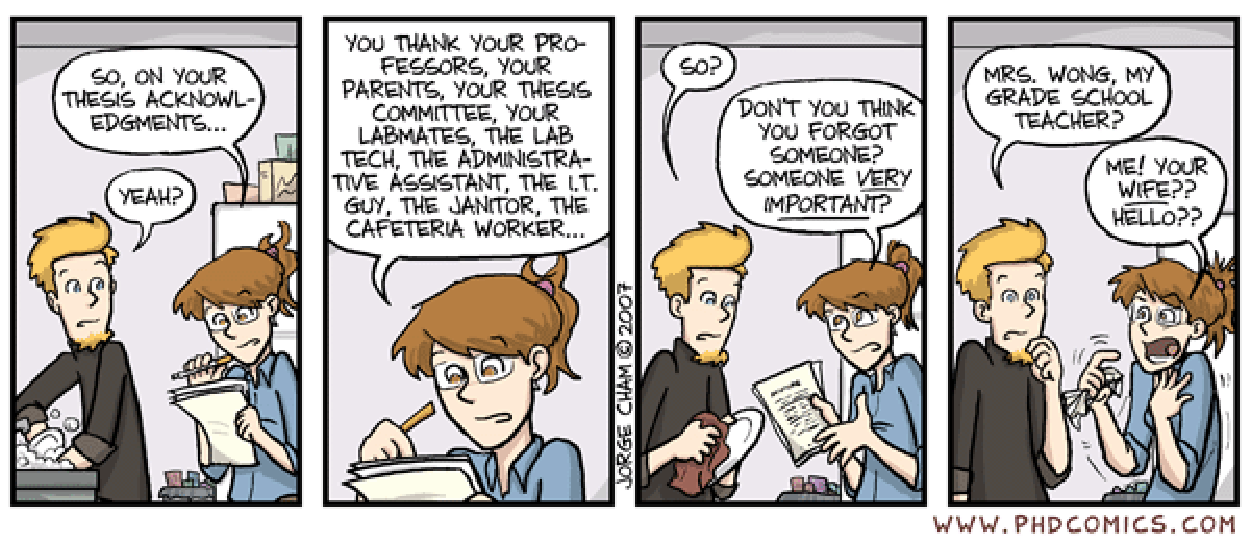
\includegraphics[width=.9\linewidth]{./graphics/phd060607s}\footnote{Source: 
%\url{http://phdcomics.com/}, no.~870 and 871}

%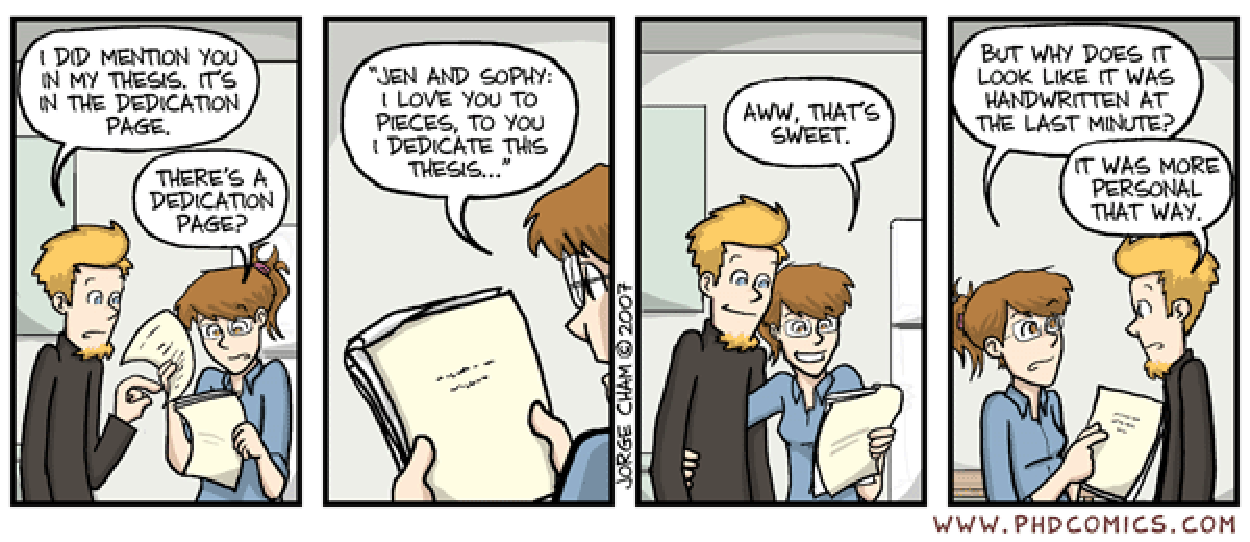
\includegraphics[width=.9\linewidth]{./graphics/phd060807s}
%\end{center}



%You should probably use \texttt{\textbackslash chapter*} for
%acknowledgements at the beginning of a thesis and
%\texttt{\textbackslash chapter} for the end.

%%% Local Variables: 
%%% mode: latex
%%% TeX-master: "../mythesis"
%%% End: 


\tableofcontents

\mainmatter
\pagestyle{scrheadings}

% Turn off DRAFT for the following pages
\ifthenelse{\equal{\ThesisVersion}{Draft}}{%
  \ifthenelse{\texlive < 2013}{%
    \SetBgContents{}
  }{%
    \backgroundsetup{contents={}}
  }
}{}

%------------------------------------------------------------------------------
% Add your chapters here - don't forget to also add them to \includeonly above
%==============================================================================
\chapter{Introduction}
\label{sec:intro}
%==============================================================================

\epigraph{Our mistake is not that we take our theories too seriously, but that 
we do not take them seriously enough.}{Steven Weinberg 
\cite{Weinberg1993first}}

Although widely accepted, Hawking radiation remains a field of heated 
discussion and active research, especially in the interpretation and 
extrapolation of it. Being one of the first conclusions of the original 
calculation, Hawking temperature was deduced from a \emph{pure state} of the 
quantum field in the background space-time of a collapsing body, whereas a 
temperature in statistical physics is usually derived from a statistical 
ensemble in equilibrium, described by a \emph{thermal} and \emph{mixed state}. 
This discrepancy itself has since long been largely ignored, albeit related 
issues have always been in spotlight, for instance the \emph{information loss 
problem} , the \emph{origin of black hole entropy} \cite{Mann2015,Harlow2016}, 
etc. A detailed investigation of the pure and thermal descriptions would help 
understanding the aforementioned questions by laying them on a more solid 
foundation.

In this work, which is motivated by \cite{Kiefer2001,Hsu2009}, the focus is to 
reveal and quantify the difference between the two cases mentioned above. 
\Cref{chap:hawrad} is a review of Hawking radiation in the 
$\rbr{3+1}$-dimensional Einstein gravitation which is basically along 
\citeauthor{Hawking1976}'s original line, as well as that in 
$\rbr{1+1}$-dimensional dilaton gravity, also known as the  
Callan--Giddings--Harvey--Strominger (CGHS) model, in which the quantum field 
theory in curved space-time not only can be \emph{derived} from the full theory 
of quantum gravity, but also be solved exactly. Then in \cref{chap:corr_field}, 
motivated by the coincidence of the particle-number expectations, which are the 
diagonal elements of the density operators, the author computes the correlator 
of field strength, so as to reveal the difference in the off-diagonal elements. 
In \cref{chap:quantifing}, inspired by a new foundation of statistical physics, 
which is based on exact results in quantum information theory, the author 
quantifies the discrepancy between the two cases by calculating the trace 
distance between them, and the results are shown to be in accordance with the 
quantum-informational foundation, as well as those in \cref{chap:corr_field}. 
\Cref{chap:summary} is summary and outlook.

In the appendices, \cref{sec:1+1ddlt} explains more details about the CGHS 
model, \cref{chap:harosc} collects some useful results in quantised simple 
harmonic oscillator, and \cref{chap:distappd} introduces trace distance and 
fidelity.

Throughout the text, the \emph{natural units} will be used unless specified, 
where the speed of light in vacuum $\lc$, the reduced Planck constant $\phs$ and 
Boltzmann constant $\bk$ are all set to unity, while the Newton constant $\nG$ 
is kept.




%%% Local Variables: 
%%% mode: latex
%%% TeX-master: "../mythesis"
%%% End: 

% Uncomment the following command to get references per chapter.
% Put it inside the file or change \include to \input if you do not want the references
% on a separate page
\printbibliography[heading=subbibliography]

%------------------------------------------------------------------------------
% Use biblatex for the bibliography
% Add bibliography to Table of Contents
% Comment out this command if your references are printed for each chapter.
% \printbibliography[heading=bibintoc]

%------------------------------------------------------------------------------
% Include the following lines and comment out \printbibliography if
% you use BiBTeX for the bibliography.
% If you use biblatex package the files should be specified in the preamble.
% \KOMAoptions{toc=bibliography}
% {\raggedright
%   \bibliographystyle{../refs/atlasBibStyleWithTitle.bst}
%   % \bibliographystyle{unsrt}
%   \bibliography{./thesis_refs,../refs/standard_refs-bibtex}
% }

%------------------------------------------------------------------------------
\appendix
% \part*{Appendix}
% Add your appendices here - don't forget to also add them to \includeonly above
%------------------------------------------------------------------------------
%\chapter{Useful information}
%\label{sec:app}
%------------------------------------------------------------------------------

In the appendix you usually include extra information that should be
documented in your thesis, but not interrupt the flow.

%\chapter{Classical gravitations}

\section{Einstein gravitation}

\section{Dilaton gravitation}

%\chapter{Quantum aspects of gravitation}

\section{Quantum fields with Einsteinian background}

\section{Quantized dilaton gravitation}

%%% Local Variables: 
%%% mode: latex
%%% TeX-master: "../mythesis"
%%% End: 

\printbibliography[heading=subbibliography]

%------------------------------------------------------------------------------
% Declare lists of figures and tables and acknowledgements as backmatter
% Chapter/section numbers are turned off
\backmatter

\listoffigures
\listoftables

%------------------------------------------------------------------------------
% Print the glossary and list of acronyms
% \printglossaries

%------------------------------------------------------------------------------
% You could instead add your acknowledgements here - don't forget to
% also add them to \includeonly above
% %------------------------------------------------------------------------------
\chapter{Acknowledgements}
\label{chap:ack}
%------------------------------------------------------------------------------

I would like to acknowledge the Bonn-Cologne Graduate School for Physics and 
Astronomy, the Rheinische Friedrich-Wilhelms-Universität Bonn, the Universität 
zu Köln and my parents, who supported my Master study financially.

I am also grateful to Prof.\ Dr.\ Claus Kiefer, Prof.\ Dr.\ Hans-Peter Nilles 
and Prof.\ Dr.\ Friedrich W. Hehl, who gave me instructions into Gravity and 
guided my thesis carefully.

I would also like to thank my fellow group members: Branislav Nikolić, Nick 
Kwidzinski, Anton Krieger, David Wichmann, Dennis Piontek, Anirudh Gundhi and 
Matthias Dahlmanns, who helped me developing the ideas as well as commenting 
the thesis.

%\begin{center}
%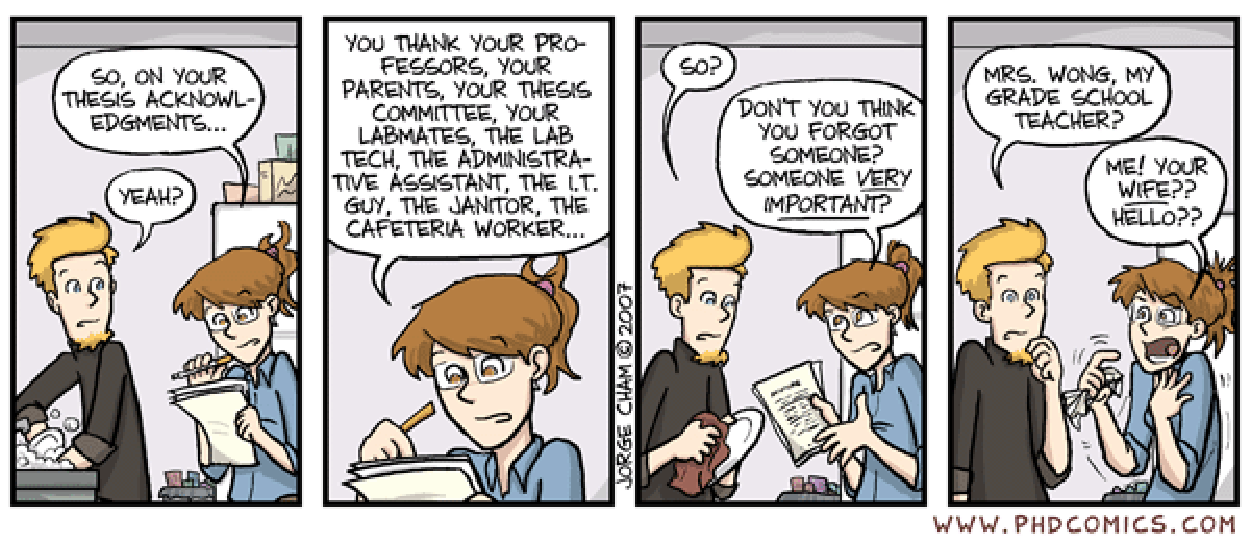
\includegraphics[width=.9\linewidth]{./graphics/phd060607s}\footnote{Source: 
%\url{http://phdcomics.com/}, no.~870 and 871}

%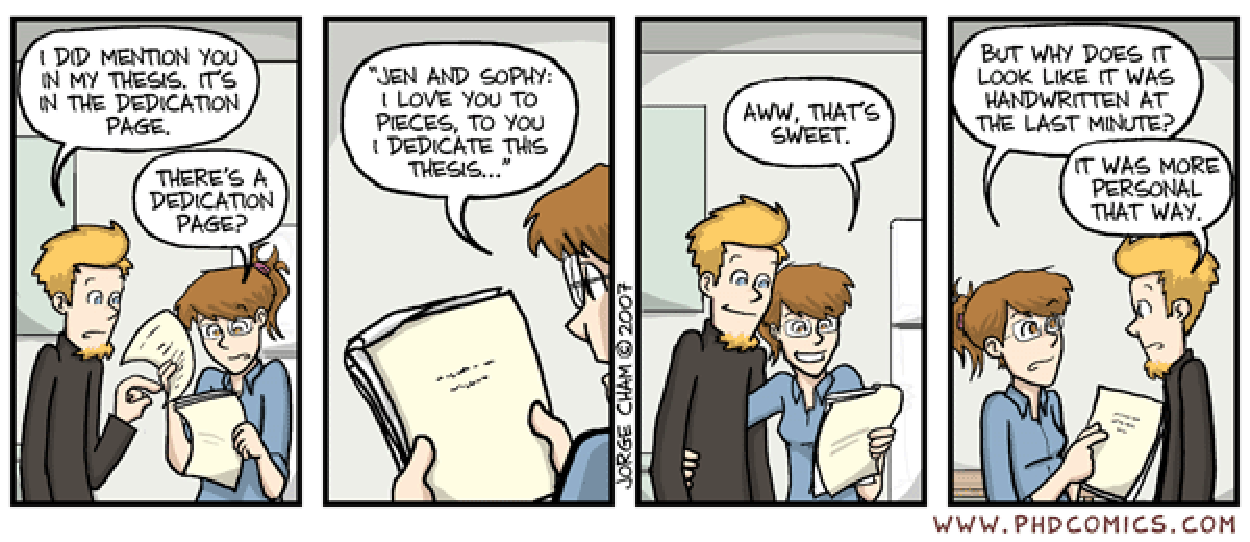
\includegraphics[width=.9\linewidth]{./graphics/phd060807s}
%\end{center}



%You should probably use \texttt{\textbackslash chapter*} for
%acknowledgements at the beginning of a thesis and
%\texttt{\textbackslash chapter} for the end.

%%% Local Variables: 
%%% mode: latex
%%% TeX-master: "../mythesis"
%%% End: 


%------------------------------------------------------------------------------
% CV needed when you submit your PhD thesis
% \definecolor{lightgray}{gray}{0.8}
\newcolumntype{L}{>{\raggedleft}p{0.15\textwidth}}
\newcolumntype{R}{p{0.8\textwidth}}
\newcommand\VRule{\color{lightgray}\vrule width 0.5pt}

\thispagestyle{empty}
\section*{Curriculum Vitae}

\subsection*{Personal Details}

\begin{tabular}{L!{\VRule}R}
Name & YiFan Wang 王一帆 \\
Date of Birth & 27.05.1990 \\
Email & yfwang@thp.uni-koeln.de \\
Family status & Single
\end{tabular}

\subsection*{Education}

\begin{tabular}{L!{\VRule}R}
%2006--2009 & Abitur, ABC Secondary School, Hamburg, Germany\\
2009--2014 & BSc in Physics, Peking University, Beijing, China.\\
2014--2017 &  MSc in Physics, Rheinische Friedrich-Wilhelms-Universität, Bonn, 
Germany. \\
\end{tabular}

\subsection*{Professional Experience}

\begin{tabular}{L!{\VRule}R}
2013 & DESY Summer Student, Zeuthen, Germany. \\
2006 & Master thesis at Universit\"at zu K\"oln, Cologne, Germany. \\
\end{tabular}

\subsection*{Languages}
\begin{tabular}{L!{\VRule}R}
Mandarin & Mother tongue
English & C1 \\
German & B2 \\
\end{tabular}


\end{document}

%%% Local Variables:
%%% mode: latex
%%% TeX-master: t
%%% End:
